\documentclass[12pt, a4paper, titlepage, hidelinks]{scrreprt}	
%% UTF-8 File Encoding
\usepackage[utf8]{inputenc}
\usepackage[T1]{fontenc}

%% Language settings
\usepackage[ngerman]{babel}

\usepackage{fullpage}
\usepackage{graphicx}
\usepackage{caption}
\usepackage{subcaption}
\usepackage{placeins}
\usepackage{wrapfig}
\usepackage{url}
\usepackage[raiselinks=true, bookmarks=true, bookmarksopenlevel=1, bookmarksopen=true, bookmarksnumbered=true, hyperindex=true, plainpages=false, pdfpagelabels=true]{hyperref}
\usepackage{fancyhdr}
\usepackage[nottoc]{tocbibind}
\usepackage[usenames, dvipsnames]{color}
\usepackage{xcolor}
\usepackage{textcomp} 
\usepackage{fancybox}
\usepackage{mathtools}
\usepackage{csquotes}
\usepackage{dirtree}
\usepackage{sidecap}
\sidecaptionvpos{figure}{t}

\usepackage{pdflscape}
\usepackage{rotating}

\usepackage{tikz}
\usetikzlibrary{arrows, positioning, fit}

\graphicspath{{images/}}

\usepackage{setspace}
\setstretch{1.4}

\usepackage[a4paper]{geometry}
\geometry{left=3.25cm,right=2.5cm,top=3.5cm,bottom=3.5cm,head=14.5pt,headsep=4ex}

\usepackage[pdftex]{thumbpdf}
\pdfcompresslevel=9

\setcounter{secnumdepth}{3}
\setcounter{tocdepth}{3}

\parindent 0cm
\parskip1.5ex plus0.5ex minus0.5ex
\clubpenalty = 10000
\widowpenalty = 10000
\displaywidowpenalty = 10000

%% Caption configurations
\usepackage{caption}
\DeclareCaptionFont{white}{\color{white}}
\DeclareCaptionFormat{listing}{\colorbox{gray}{\parbox{\textwidth}{#1#2#3}}}
\captionsetup{font=small}
%\captionsetup[lstlisting]{format=listing,labelfont=white,textfont=white}
\definecolor{lightgray}{rgb}{.9,.9,.9}
\definecolor{darkgray}{rgb}{.4,.4,.4}
\definecolor{purple}{rgb}{0.65, 0.12, 0.82}

%% Contents in pdf bookmark list
%% uses etoolbox
\makeatletter
\pretocmd{\tableofcontents}{%
  \if@openright\cleardoublepage\else\clearpage\fi
  \pdfbookmark[0]{\contentsname}{toc}%
}{}{}%
\makeatother

\usepackage{lmodern}

\usepackage[activate={true,nocompatibility},final,tracking=true,kerning=true,spacing=true,factor=1100,stretch=10,shrink=10]{microtype}
\microtypecontext{spacing=nonfrench}

\pagestyle{fancy}
\renewcommand{\chaptermark}[1]{\markboth{\thechapter.\ #1}{}}
\fancyhf{}
\fancyhead[LE,RO]{{\headfont\thepage}}
\fancyhead[LO]{\headfont\nouppercase{\rightmark}}

%% better syntax highlighting
\usepackage[chapter, outputdir=out]{minted}
\usemintedstyle{colorful} %https://raw.github.com/n1k0/SublimeHighlight/master/themes.png
\newcommand{\mintedfileinput}[2]{
\microtypesetup{protrusion=false}
\inputminted[frame=lines,framesep=7pt,linenos=false,numbersep=6pt,baselinestretch=1,xleftmargin=10pt, tabsize=2]{#1}{"../#2"}
\microtypesetup{protrusion=true}
}

\newcommand{\mintedfile}[4]{
\begin{listing}[H]
  \mintedfileinput{#1}{#2}
  \vspace{-16pt}
  \caption{#3}
  \label{#4}
\end{listing}
\vspace{-17pt}
}

\newcommand{\imagewrap}[4][R]{
\begin{wrapfigure}{#1}{#2\textwidth}
  \vspace{-20pt}
  \begin{center}
    \includegraphics[width=#2\textwidth]{#3}
  \end{center}
  \vspace{-20pt}
  \caption{#4}
  \label{#3}
  \vspace{-15pt}
\end{wrapfigure}
}

\hypersetup{
 pdfauthor={Mathias Garbe},
 pdftitle={Labor Algorithmen Dokumentation},
 pdfsubject={},
 pdfkeywords={}
}

\title{Labor Algorithmen - Sortierverfahren}
\subtitle{Dokumentation}
\author{Mathias Garbe}

\begin{document}

\pagenumbering{roman}
\maketitle

\microtypesetup{protrusion=false}
\tableofcontents
\microtypesetup{protrusion=true}

\clearpage

\pagenumbering{arabic}

\chapter{Sortieralgorithmen}

\section{Insertion Sort}

Der Insertion Sort Algorithmus ist ein leicht zu implementierendes und stabiles Sortierverfahren. Es nimmt aus der unsortierten Folge ein Element und fügt es vorne an richtiger Stelle der Folge wieder ein (daher auch \textit{Insertion Sort}), wobei die übrigen Elemente der Folge beim Einfügen nach hinten verschoben werden müssen. Dies wird nun an jeder Stelle der Folge von Anfang bis Ende durchgeführt bis die Folge sortiert ist. Der große Teil des Aufwands beim Insertion Sort liegt hierbei im Finden der richtigen Einfügeposition und das Verschieben der übrigen Elemente.

\paragraph{Variation: Wächterelement} Bei dieser Variation wird das kleinste Element vor dem Sortieren mit dem Insertion Sort Algorithmus an die erste Stelle der Folge verschoben. Dieses Element wird auch \textit{Wächterelement} genannt. Somit kann im Rumpf des Algorithmus die Abfrage auf ein Unterschreiten der Folge eingespart werden, was gegebenenfalls die Laufzeit reduzieren kann.

\paragraph{Variation: Wächterelement und Indextransformation} Zusätzlich zum Wächterelement wird hierbei die Berechnung des neuen Indexes an den Anfang der Schleife verschoben und somit kann gegebenenfalls die Laufzeit reduziert werden, da der neue Index nur einmal anstatt mehrmals berechnet werden muss.

\clearpage

\begin{SCfigure}
  \centering
  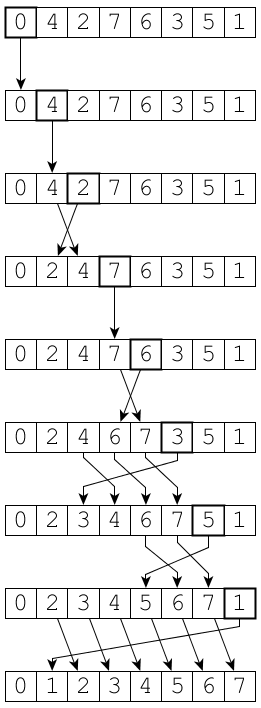
\includegraphics[width=0.5\textwidth]{graphs/Insertion-Sort.png}
  \caption*{\textbf{Schritt 1}: Das erste Element wird als sortiert angenommen und übersprungen. \\[45pt] %
  	\textbf{Schritt 2}: Das zweite Element wird überprüft und ist an der richtigen Stelle der Folge. \\[40pt] %
  	\textbf{Schritt 3}: Die \textit{2} ist nicht an der richtigen Stelle und muss nach an der zweite Stelle eingefügt werden. Alle nachfolgenden Elemente müssen verschoben werden. \\[15pt] %
  	\textbf{Schritt 4}: Das vierte Element wiederum muss nicht verschoben werden. \\[42pt] %
  	\textbf{Schritt 5}: Hier muss nun die \textit{6} vor die \textit{7} an der vierten Stelle eingefügt werden und alle nachfolgenden Elemente verschoben werden. \\[28pt] %
  	\textbf{Schritt 6}: Auch hier wird muss \textit{3} weit am Anfang eingefügt und viele nachfolgende Elemente verschoben werden.\\[32pt] %
  	\textbf{Schritt 7}: Die \textit{5} wird an der fünften Stelle eingefügt und alle nachfolgenden Elemente verschoben. \\[26pt] %
  	\textbf{Schritt 8}: Das letzte Element muss nun an der zweiten Position eingefügt werden, und beinahe die komplette Folge muss verschoben werden. \\[16pt] %
  	\textbf{Schritt 9}: Die Folge ist nun vollständig sortiert.
  }
\end{SCfigure}
\clearpage
\section{Quicksort}

Im Durchschnitt kommt Quicksort mit $\mathcal{O}(n\log{}n)$ Vergleichen aus, im schlimmsten Fall $\mathcal{O}(n^2)$. In der Praxis ist Quicksort meist schneller als andere $\mathcal{O}(n\log{}n)$ Algorithmen. Auch sein sequentieller Speicherzugriff zusammen mit seiner sehr kurzen Schleife ist prädestiniert um von dem Prozessorcache zu profitieren.

\paragraph{Beispiel} 
\imagewrap{0.4}{graphs/quicksort.png}{Quicksort Beispiel}
\textbf{Schritt 1:} Als Pivot wird der Mittelpunkt der Folge genommen, hier die \textit{7}. Alle Werte kleiner als des Pivots werden auf die linke Seite verschoben, alle Werte größer des Pivots auf die rechte Seite. Danach wird die Folge in der Mitte (nach der 7) partitioniert.

\textbf{Schritt 2 und Schritt 3:} Für alle Partitionen wird Schritt 1 wiederholt bis jede Partition nur noch aus einem Element besteht.

\textbf{Schritt 4:} Jede Partition besteht nur noch aus einem Element. Die Folge ist demnach vollständig sortiert.

\paragraph{Variation: Shiftoperator statt Division} Bei dieser Variante wird die Mitte der Partition nicht durch eine Division durch 2 ermittelt sondern durch einen Rechtsshift um 1.

\paragraph{Variation: 3-way-partitioning mit Shiftoperator}

\paragraph{Variation: Hybrider Ansatz}
\section{Mergesort}
Das Mergesort Sortierungsverfahren arbeitet nach dem Prinzip des \textit{teilen und herrschen} (\textit{divide and conquer}). Auch dieser Algorithmus sortiert Folgen stabil. Es betrachtet die unsortierte Folge als eine Liste von Teilfolgen, welche am Anfang nur ein Element besitzen. Diese Teilfolgen werden dann im Reißverschlussverfahren zu größeren Folgen zusammengefügt (das \textit{mergen}). Dabei kann Mergesort davon ausgehen, dass jede Teilfolge sortiert ist. Dies ist im ersten Schritt sichergestellt, da jede Teilfolge nur aus ein Element besteht und somit schon sortiert ist. Um nun zwei sortierte Teilfolgen zusammenzufügen müssen diese Teilfolgen jeweils von links nach rechts durchgegangen werden und jeweils der kleinere Wert aus der Teilfolge genommen und in die neue Folge hinten angefügt werden. Dies wird solange wiederholt, bis beide Teilfolgen leer sind. Somit entsteht eine neue, sortierte Folge. Wird dies nun für alle Teilfolgen wiederholt bis es nur noch eine Folge gibt so ist diese gesamte Folge sortiert.

Die Arbeit des Aufteilen einer unsortierten Folge ist trivial, das eigentliche Zusammenfügen ist bei Mergesort jedoch die eigentliche Arbeit. Auch kann Mergesort nur sehr aufwändig ohne einen temporären Speicher ausgeführt werden (\textit{in-place}) und ist somit in der Regel auf den Speicherplatz einer zweiten, gleichgroßen Folge angewiesen.

Mergesort benötigt sowohl im durchschnitt als auch im besten und schlechtesten Fall stets $\mathcal{O}(n\log{}n)$ Vergleiche.

\paragraph{Beispiel}
\imagewrap{0.4}{graphs/mergesort.png}{Mergesort}

\paragraph{Variation: Natural Mergesort} Bei dem Natural Mergesort wird zuerst versucht natürlich vorkommende Teilstücke in der Folge zu finden, die bereits sortiert sind. Durch das Ausnutzen dieser Sortierung lässt sich gegebenenfalls Schritte des Mergesorts einsparen. Es können dabei sowohl aufsteigend als auch absteigend sortierte Teilfolgen benutzt werden (\textit{Bitonische Läufe}).

\chapter{Zeitmessungen}
Die Zeiten der einzelnen Messungen sind Durchschnittswerte von fünf unabhängigen Läufen mit jeweils unterschiedlichen Zufallsfolgen. Dabei wird pro Lauf jeder Algorithmus mit den gleichen Zufallsfolgen getestet. Die auf- und absteigenden Folgen unterscheiden sich nicht zwischen den Läufen.

\begin{table}[h]
\begin{tabular}{|l|l|l|l|l|l|l|l|l|l|l|l|l|}
\hline
 & 10000 & 20000 & 40000 & 80000 & 160000 & 320000 & 640000 & 1280000 & 2560000 & 5120000 & 10240000 & 20480000 \\ \hline
InsertionSort & 13 & 52 & 207 & 857 & 3496 & 17417 & 57109 & - & - & - & - & - \\ \hline
InsertionSortGuard & 19 & 77 & 313 & 1039 & 4152 & 21865 & 72085 & - & - & - & - & - \\ \hline
InsertionSortGuardTr. & 14 & 56 & 228 & 949 & 3839 & 19893 & 65926 & - & - & - & - & - \\ \hline
MergeSortTopDown & 4 & 7 & 15 & 31 & 62 & 127 & 264 & 532 & 1071 & 2183 & 4441 & 9083 \\ \hline
MergeSortBottomUp & 0 & 1 & 3 & 7 & 14 & 32 & 66 & 143 & 300 & 621 & 1313 & 2702 \\ \hline
MergeSortNatural & 0 & 2 & 3 & 7 & 16 & 33 & 72 & 154 & 325 & 683 & 1431 & 2980 \\ \hline
QuickSort & 0 & 1 & 2 & 4 & 10 & 21 & 43 & 91 & 193 & 400 & 837 & 1725 \\ \hline
QuickSortShift & 0 & 1 & 2 & 5 & 9 & 21 & 43 & 92 & 192 & 400 & 835 & 1727 \\ \hline
QuickSortShift3Way & 0 & 1 & 2 & 5 & 10 & 22 & 46 & 96 & 203 & 423 & 884 & 1822 \\ \hline
QuickSort3WayHybrid & 0 & 1 & 2 & 5 & 11 & 24 & 50 & 105 & 221 & 463 & 962 & 2064 \\ \hline
Heapsort & 0 & 1 & 2 & 5 & 13 & 29 & 72 & 198 & 581 & 1614 & 4140 & 10209 \\ \hline
\end{tabular}
\caption{Zufallswerte (Zeiten in Millisekunden)}
\end{table}
\begin{table}[h]
\begin{tabular}{|l|l|l|l|l|l|l|l|l|l|l|l|l|}
\hline
 & 10000 & 20000 & 40000 & 80000 & 160000 & 320000 & 640000 & 1280000 & 2560000 & 5120000 & 10240000 & 20480000 \\ \hline
InsertionSort & 0 & 0 & 0 & 0 & 0 & 0 & 1 & - & - & - & - & - \\ \hline
InsertionSortGuard & 0 & 0 & 0 & 0 & 0 & 0 & 1 & - & - & - & - & - \\ \hline
InsertionSortGuardTr. & 0 & 0 & 0 & 0 & 0 & 0 & 1 & - & - & - & - & - \\ \hline
MergeSortTopDown & 3 & 6 & 13 & 27 & 53 & 108 & 224 & 447 & 897 & 1818 & 3678 & 7508 \\ \hline
MergeSortBottomUp & 0 & 0 & 1 & 3 & 6 & 13 & 28 & 67 & 140 & 292 & 611 & 1289 \\ \hline
MergeSortNatural & 0 & 0 & 0 & 0 & 0 & 0 & 1 & 3 & 7 & 16 & 32 & 64 \\ \hline
QuickSort & 0 & 0 & 0 & 1 & 2 & 4 & 8 & 18 & 38 & 81 & 170 & 353 \\ \hline
QuickSortShift & 0 & 0 & 0 & 1 & 2 & 4 & 9 & 18 & 39 & 81 & 169 & 353 \\ \hline
QuickSortShift3Way & 0 & 0 & 0 & 1 & 2 & 4 & 8 & 18 & 37 & 77 & 161 & 334 \\ \hline
QuickSort3WayHybrid & 0 & 0 & 0 & 1 & 3 & 7 & 15 & 31 & 67 & 143 & 293 & 617 \\ \hline
Heapsort & 0 & 1 & 2 & 4 & 9 & 19 & 41 & 88 & 191 & 404 & 844 & 1764 \\ \hline
\end{tabular}
\caption{Aufsteigende Werte (Zeiten in Millisekunden)}
\end{table}
\begin{table}[h]
\begin{tabular}{|l|l|l|l|l|l|l|l|l|l|l|l|l|}
\hline
 & 10000 & 20000 & 40000 & 80000 & 160000 & 320000 & 640000 & 1280000 & 2560000 & 5120000 & 10240000 & 20480000 \\ \hline
InsertionSort & 26 & 103 & 421 & 1742 & 7041 & 35906 & 118667 & - & - & - & - & - \\ \hline
InsertionSortGuard & 39 & 153 & 618 & 2073 & 8308 & 43788 & 143994 & - & - & - & - & - \\ \hline
InsertionSortGuardTr. & 29 & 113 & 456 & 1924 & 7786 & 40625 & 136397 & - & - & - & - & - \\ \hline
MergeSortTopDown & 3 & 6 & 13 & 26 & 53 & 108 & 224 & 448 & 898 & 1838 & 3687 & 7594 \\ \hline
MergeSortBottomUp & 0 & 1 & 1 & 3 & 6 & 13 & 31 & 68 & 145 & 305 & 654 & 1342 \\ \hline
MergeSortNatural & 0 & 1 & 2 & 4 & 8 & 18 & 39 & 83 & 177 & 369 & 778 & 1605 \\ \hline
QuickSort & 0 & 0 & 0 & 1 & 2 & 4 & 9 & 19 & 40 & 85 & 177 & 372 \\ \hline
QuickSortShift & 0 & 0 & 0 & 1 & 2 & 4 & 9 & 19 & 40 & 85 & 178 & 368 \\ \hline
QuickSortShift3Way & 0 & 0 & 0 & 1 & 2 & 4 & 9 & 19 & 39 & 82 & 169 & 353 \\ \hline
QuickSort3WayHybrid & 0 & 0 & 0 & 1 & 3 & 7 & 15 & 31 & 66 & 141 & 289 & 614 \\ \hline
Heapsort & 0 & 1 & 1 & 4 & 9 & 18 & 40 & 88 & 193 & 416 & 882 & 1859 \\ \hline
\end{tabular}
\caption{Absteigende Werte (Zeiten in Millisekunden)}
\end{table}


\end{document}
